\subsection{Decision Tree Feature Generation}

\subsubsection{MNIST}

In working with the decision trees, we utilized the SVD of each image in the training set. 


\subsection{LDA vs PCA}

LDA and PCA linearly transforms the data to reduce the dimensions. The difference is LDA is supervised whereas PCA is unsupervised. PCA finds directions which maximize the variance along that direction and they are orthogonal to each other. We can view a PCA technique as in Figure(2.1). 

	\begin{figure}[H]
		\centering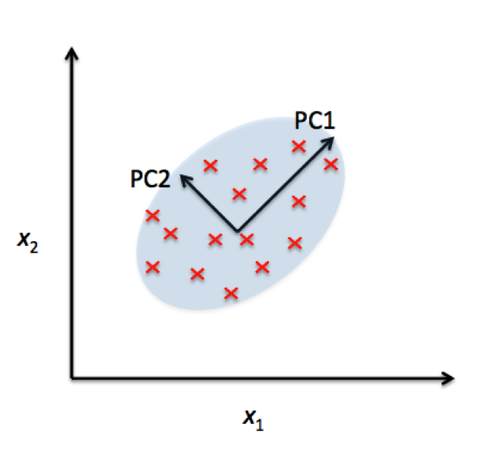
\includegraphics[width=0.6\textwidth]{../images/pca}
		\caption{PCA implemented on 2-dimensional data}
	\end{figure}

LDA maximizes the class separability and can be viewed as in Figure(2.2). 
	\begin{figure}[H]
	\centering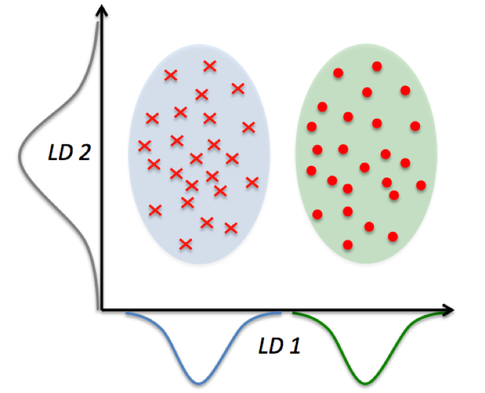
\includegraphics[width=0.6\textwidth]{../images/lda}
	\caption{LDA visualization}
	\end{figure}

\subsection{LDA for MNIST and Extended YaleB}
LDA reduces the data with K classes with large dimensions to K-1 dimensions which captures the most energy of the data. Implementing LDA as a dimension reduction, MNIST and Extended YaleB datasets are reduced to 9 and 37 variables for each data point. Then we worked with this transformed data to do further classification. 
